\documentclass[conference,compsoc]{IEEEtran}
\usepackage{ifpdf}
\usepackage{caption}
\usepackage[pdftex]{graphicx}
\usepackage[noadjust]{cite}
\usepackage{amsmath}
\usepackage{enumitem}
\usepackage[caption=false,font=footnotesize,labelfont=sf,textfont=sf]{subfig}
\usepackage{fixltx2e}
\hyphenation{op-tical net-works semi-conduc-tor}
\renewcommand{\citedash}{--}

\setlist[itemize]{leftmargin=*}

\begin{document}

\title{Visual Dataflow Language for Educational Robots Programming}

\author{
	\IEEEauthorblockN{Grogorii Zimin}
	\IEEEauthorblockA{
		Mathematics and Mechanics Faculty,\\
		SPbSU\\
		Saint-Petersburg, Russia \\
		Email: zimin.grigory@gmail.com
	}
	\and

	\IEEEauthorblockN{Dmitrii Mordvinov}
	\IEEEauthorblockA{
		Mathematics and Mechanics Faculty,\\
		SPbSU\\
		Saint-Petersburg, Russia \\
		Email: mordvinov.dmitry@gmail.com
	}
}

\maketitle



\begin{abstract}
The paper describes a novel dataflow visual programming environment for embedded robotic platforms. Its purpose is to be bridge between lightweight educational robotic programming languages and complex industrial languages. We compare programming environments mostly used by robotics community with our tool. A brief review of behavioural robotic architectures and some thoughts on expressing them in terms of our language are given. We also provide the examples of solving two typical robot contol tasks in our language.
\end{abstract}

\section{Introduction}

Programming languages for creating robotic controllers are actual topics of research oftenly discussed at major conferences, such as ICRA\cite{Icra} or IROS\cite{Iros2016}. Visual programming languages (VPLs) are also actively discussed for the last three decades, the largest conferences are held annually, e.g. VL/HCC\cite{VLHCC}. VPLs are oftenly applied in robotics domain\cite{banyasad2000visual,simpson2006mobile,simpson2008visual,posso2011process,diprose2011ruru} allowing to create and visualize robotic controllers. Robotic VPLs are commonly used for educational purposes, making possible for students of even junior schools to create robotic programs. There already exists a great number of educational robotic programming environments based on VPLs, e.g. NXT-G\cite{nxtg}, TRIK Studio\cite{trik}, ROBOLAB\cite{robolab}, also there are some academic tools implementing interesting and novel approaches to educational robotics programming\cite{banyasad2000visual,simpson2008visual,diprose2011ruru}.

Robotic control programs are inherently reactive: they transform data which is continuously coming from multiple sensors into the impulses on actuators. For this reason dataflow languages (DFLs) are well-suitable for robotics programming. Many researchers denoted the conveniency of dataflow visual programming languages (DFVPLs)\cite{johnston2004advances}, finding them more useful than textual DFLs, for example because data flows explicitly displayed on the diagram. There are large and complex general-purpose and domain-specific development environments such as LabVIEW\cite{labview} and Simulink\cite{simulink} that provide a large (and sometimes even cumbersome) set of libraries for robotics programming. More detailed discussion of robotics VPLs will be provided in section~\ref{sec:Overview}.

There is a large number of robotic constructor kits for learning the basics of robotics and cybernetics, such as LEGO MINDSTORMS\cite{legokit}, TRIK, ScratchDuino\cite{ScratchDuino}. Modern programming languages that are used for programming those kits are based on the control flow model rather than on dataflow model. Control flow-based languages are good for solving scholar ``toy'' tasks, but may be inconvenient for programming more complex ``real world'' controllers that may be conveniently expresses on DFLs. The simple DFVPL may be considered as a useful step from educational VPLs to the programming languages that are used in unversities and industry. 


This paper discusses a novel extensible tool for programming all popular educational robotic kits on dataflow visual programming language. One of the most important distinction of our tool from others is its focus on embedded systems (section~\ref{sec:Implementation}). Another interesting detail of our work is the application of DSM-aproach for implementation of visual editor: it is entirely generated by QReal DSM-platform\cite{qrealMeta}\cite{kuzenkova2013qreal} without even a line of code written. We also take into consideration the popularity of Brooks' Subsumption Architecture\cite{brooks1986robust} which is still mainstream aproach to design of complex robotic controllers\cite{banyasad2000visual,simpson2006mobile,posso2011process,proetzsch2007behaviour} despite it was proposed 30 years ago. Brooks' Subsumption Architecture and some other are conveniently expressed in our language, they are discussed in section~\ref{sec:Architectures}.

The remainder of a paper is organized as follows. An overview of robotics VPLs and DFVPLs is presented in section~\ref{sec:Overview}. Section~\ref{sec:Architectures} provides some general thoughts on how some widely used robotic behavioural acrhitectures are expressed in our language. A detailed description of our language is given in section~\ref{sec:lang}. Section~\ref{sec:example} demonstrates two typical robotic controllers expressed in our language. The most important details of implementation are deiscussed in section~\ref{sec:Implementation}. Finally, the last section concludes the paper and discusses possible directions for future work.


\section{Similar Tools}
\label{sec:Overview}
Robot programming environments can be divided into three categories: educational, which allows to program small educational robotic kits; industrial, which have a rich toolkit for creating large and complex robotic controllers; academic, which implement new interesting ideas, however they are oftenly unavailable for downloading or unusable.

Educational visual enviroments are for example NXT-G and ROBOLAB for LEGO MINDSTORMS NXT kit, EV3 Software for the Lego Mindstorms EV3 kit, TRIK Studio for NXT, EV3 and TRIK. Those environments simplify solving primitive robot control tasks like finding a way out of the maze and driving along the line using light sensors, which makes the process of learning the basics of programming and robot control easy. But their simplicity oftenly bounds the flexibility of the language. Visual languages of all mentioned systems are based on control flow model.

There is also a number of well-known visual robotic programming environments of industrial level. For example, general-purpose LabVIEW from National Instruments with the DFVPL G, programming environment Simulink developed by MathWorks for modeling different dynamic models or control systems. Those products offer to a huge set of models and libraries to create control systems, test benches, real-time systems of any complexity, using model-driven approach. LabVIEW provides opportunity for programming small robots. There are lots of examples of applying LabVIEW in education\cite{erwin2000lego, 1_gomez-de-gabriel_mandow_fernandez-lozano_garcia-cerezo_2011}, but much more oftenly its adaptations like Robolab are used in educational process. It should be noted that those environments are distributed under the commercial license.

Another example of an visual robotics industrial system is the Microsoft Robotics Developer Studio (MSRDS)\cite{jackson2007microsoft}, which is free for academic purposes and allow to create distributed robotic systems on DFVPL. MSRDS officially supports a large set of robotic platforms, LEGO NXT\cite{kim2007programming} in particular (however, the autonomious mode for NXT is not supported). MSRDS has the ability of manual integration with custom robotic platforms, but unhappily is not maintained since 2014.

There is a lot of scientific research done in this area, e.g., dissertation\cite{banyasad2000visual} describes a visual programming module for expressing robotic controllers in terms of extended Moore machines, \cite{simpson2008visual, posso2011process} describe visual environment for $occam\mbox{-}\pi$ language and $Transterpreter$ framework, and its usage in education and swarm robotics. Article\cite{diprose2011ruru} describes DFVPL for beginners which is pretty close to a one we introduce here. However at the moment RuRu is under development, it has pretty limited functionality and even unavailable for download.

\section{Robotic Behavioural Architectures}
\label{sec:Architectures}

The task of creation complex and scalable robotic controller is indeed a non-trivial task. Starting from middle 80's many researchers have attempted to solve this problem and a number of behavioural robotic architectures were proposed\cite{simpson2009toward}. Those aproaches are quickly became popular in robotics community and they are still actual. For example the original work that introduced Brooks' \textit{Subsumption Architecture}\cite{brooks1986robust} is one of the most cited works in the entire robotics domain. We believe that the description of modern language for programming robotic controllers should contain at least general thoughts on how those architectures may be expressed in it.

A controller built on Brooks' Subsumption Acrhitecture is decomposed into a hierarchy of levels of competence where each new layer describes a new feature of robot's behaviour. Levels are ``ordered'' upside-down, the higher levels describe more ``intelligent''  behaviour of robot. Higher levels depend on lower ones but not vice versa, so failures of higher levels do not imply the failure of lower. This is important feature for mobile robotics, e.g. if robot's gripper was damagged the controller is still able to deliver robot to its base. Levels of responsibility are expressed as a set ``behaviours'' running concurrently and interacting with each other via channels of \textit{suppression} and \textit{inhibition}. Using them higher levels can suppress the activity of lower ones thus correcting the behaviour of the whole system.

Brooks' in his original work offered to express behaviours in terms of \textit{state machines}. Each layer implements some simple logic of transformation sensor inputs into impulses on actuators. Dataflow languages are obviously as suitable as state machines for expressing such behaviours. In our language each behaviour can be represented as ``black box'' described by separate subprogram. Also our language contains $Suppressor$ and $Inhibitor$ elements for layers communication. Levels can be invoked concurrently, so we can conclude that our language allows the convenient expression of controllers built with Subsumption Architecture. That is demonstrated by an example in section~\ref{sec:example}.

Connell's \textit{Colony Architecture}\cite{connell1989colony} is a very similar to Brooks' one, but solves some scalability issues of Subsumtion Architecture. It also decomposes the controller into a number of communicating concurrent levels, but they are unordered. The other difference is in an absence of inhibition channel, data inhibition should be implicitly expressed by predicated in layers. Our lanuage does not force any order between layers, predicative inhibition can be implemented simply with $Filter$ block. So Colony Architecture is also well-expressed in our language.

There also exist Arkin’s \textit{Motor Schema}\cite{arkin1987motor} and Rosenblatt’s \textit{Distributed Architecture for Mobile Navigation} (\textit{DAMN})\cite{rosenblatt1997damn} which are compatible with our language, but the detailed descriptions will be omitted here. General ideas on their implementation on $occam\mbox{-}\pi$ language can be found in \cite{simpson2009toward}, we believe that those ideas will suffice in the context of this paper. The complete research of expressing behavioural architectures in our language is a topic for separate paper.


\section{Language Description}
\label{sec:lang}

Evolution of a domain-specific modeling (DSM) tools allows to quickly create a fairly sophisticated visual programming languages\cite{DSM}. TRIK Studio programming environment is an example of a system that was created using DSM-based approach on QReal platform\cite{qrealMeta, kuzenkova2013qreal}. Basing on an industrial experience of TRIK Studio developers we decided to create the visual editor of our language on QReal platform.

Program on DFVPL is a set of blocks and flows that connect blocks. DFVPL blocks process incoming tokens and emit resulting data into the output data flows. Blocks in our language can be divided into several groups that are described below. Some blocks require to specify information on textual language. The language we use is a statically typed dialect of Lua\cite{lua}.

\begin{itemize}
\item \textit{Control} blocks that implement basic algorithmic constructions (conditions, loops, etc).
\begin{itemize}
\item \textit{ConstValue} and \textit{RandomValue} blocks that are responsible for generation of a random number or a predetermined value of any type.
\item \textit{Loop, If, Switch}. These blocks implement general control flow algorithmic constructions in dataflow style. $Loop$ is an entity which emitting a sequence of numbers for a given amount of times. $If$ checks the condition specified on a textual language and sends them to $True$ or $False$ channel. $Switch$ successively checks guard conditions and if it is evaluated as $true$ sends incoming data to corresponding channel.  	
\item \textit{Function} block, which allows to process of the input data in a textual language. Most oftenly this block is used for mathematical processing of data.
\item \textit{FinalBlock} stops the execution of program when receiving any data. 
\item \textit{Subprogram} for reusing the code. Double-click on subprogram block opens new visual editor tab with an implementation of this subprogram. Contents of that tab can be then edited by user in exactly the same way he edits the main diagram.
\item \textit{GetSetVariable}. Purely practical block for setting value of some global variable or emitting it into output flows.
\item \textit{Wait} block delays data processing.
\item \textit{DelayAndFilter} is the extension of the previous block adding the filtering condition and checking the amount of emitted data validated by condition.
\item \textit{Fork, EndFork} blocks that provide an ability of invoking code in platform-specific execution units. See section~\ref{sec:Implementation} for details.
\end{itemize} 
\item \textit{Drawing}. Blocks for drawing on display of the robot and on the floor in simulator mode.
\begin{itemize}
\item \textit{PaintSettings} defines current background color, thickness and color of pen and color and style of the brush that draw graphical primitives.
\item \textit{ShapePainter, SmilePainter, Text} are used for drawing some shape, text or smile on robot's display. 
\item \textit{Clear} block removes all graphics from robot's display when receiving any token.
\item \textit{Pen} block puts down or raises the marker for drawing the robot's trace on the ``floor'' of 2D simulator.
\end{itemize} 
\item \textit{Flow manipulation}. These elements provide opportunity to manipulate data which flow between blocks.
\begin{itemize}
\item \textit{InPort, OutPort} emit tokens that come into some instance of $Subprogram$ block into a diagram implementing it and similarly redirect data from subprogram implementation into output flows of active instance of $Subprogram$ block.
\item \textit{Supressor, Inhibitor} inhibit or replace token of some flow with tokens of another. These, $Subprogram$ and $Fork$ blocks provide a compability with the Brooks' Subsumption Architecture.
\item \textit{Zip, Unzip} provide an opportunity to gather data from several $Flows$ into one and vice versa.
\end{itemize} 
\item \textit{Actions} provide an ability to query and modify state of robot's input and output devices.
\begin{itemize}
\item \textit{Sensor} continuously emits data from specified sensor, e.g. infrared, light, etc.
\item \textit{Servo, Motors} process received data and send impulses to robot actuators.
\item \textit{Encoders} block sets the motors tacho limit when receiving data and continuously emits encoder values into output flows.
\item \textit{SendMessage, ReceiveMessage} responsible for the coordination of a group of robots.
\item \textit{Say, PlayTone, LED} responsible for managing speakers and LED lights.
\item \textit{RemoveFile, WriteToFile, ReadFile} implement working with file system.
\item \textit{InitCamera, DetectByVideo, StreamingNode} wrap some algorithms of computer vision.
\item \textit{PortBlock} provides an ability to write low-level to some port of the robot.
\item \textit{SystemCall} responsible for the command execution by command line interpreter, e.g. token ``reboot'' will reboot robot.
\item \textit{Gamepad} reads data from the operator's control device, e.g. gamepad, and emits it.
\end{itemize} 
\end{itemize} 


These blocks are enough to express a pretty wide range of the robotic controllers of varying complexity. If several blocks emitting data from one input device are met only one of them is active. That detail distingushes our tool from other implementing data flow paradigm, for details see section~\ref{sec:Implementation}. For example figure~\ref{image:encoder} shows diagram with $Motors, ConstValue, Encoders, Flows$ where $Encoders$ block is presented twice. When interpretation started $ConstValue$ emits data to $Motors$ and $Encoders$ (a) emits a value of a tacho counter. When block $Encoders$ (b) receives some data and thus nullifies encoder value, at that moment $Encoders$ (a) stops emitting tokens.

\begin{figure}[ht]
	\centering
	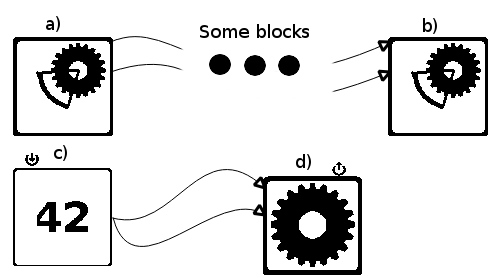
\includegraphics[width=3.5in]{Encoders.png}
	\caption{Block with many representations but only one of them can be active. a,b --- \textit{Encoders} c --- \textit{ConstValue} d --- \textit{Motors}}
	\label{image:encoder}
\end{figure}


One important detail about our language is that it explicitly supports control flow model, that is important for educational goals. On figure~\ref{image:encoder} $ConstValue$ and $Motors$ have incoming and outgoing ``arrows'', which are used to connect control flow data. For example $Motors$ block emits data to control flow channel when handle incoming data and $ConstValue$ emits its value when receives control flow token. 

Flows may be pinned to a block on left, right and bottom side, which are highlighted when user edits block (see Figure~\ref{image:block}). Also block may contain text fields, e.g. on Figure~\ref{image:block} user entered textual condition.
\begin{figure}[ht]
	\centering
	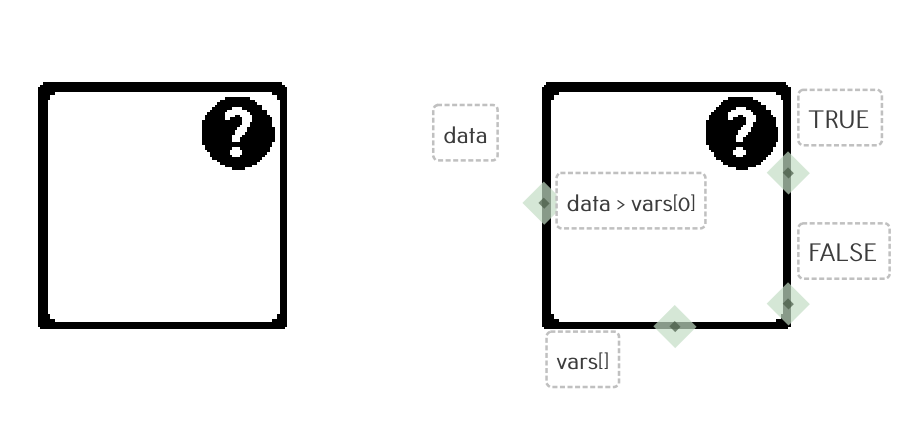
\includegraphics[width=3.5in]{block.png}
	\caption{Showing and editing of block.}
	\label{image:block}
\end{figure}



\section{Example}
\label{sec:example}
Figures~\ref{image:boxC},~\ref{image:box} show simple PD-regulator which keeps robot on a certain distance from a wall using infrared sensor. Global variable is used for storing old sensor values. Expressions in $Function$ block are calculated in upside-down order, results of previous exressions are available on lower levels. Each level emits resulting token into a corresponding flow, in our example two flows are connected directly to motors control block.


\begin{figure}[ht]
	\centering
	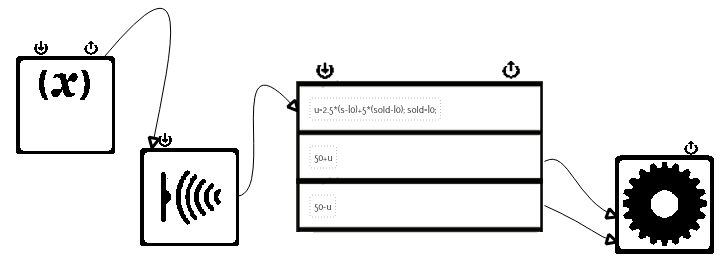
\includegraphics[width=3.5in]{alongBoxCode.png}
	\caption{Controller for the wall following.}
	\label{image:boxC}
\end{figure}

\begin{figure}[ht]
	\centering
	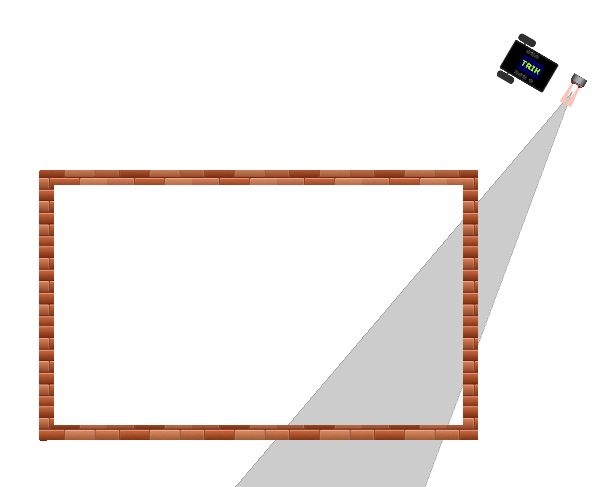
\includegraphics[width=3.5in]{alongBoxModel.png}
	\caption{Simulation process of the wall following.}
	\label{image:box}
\end{figure}

Let's describe more complex robotic controller. We have the robot equipped with two power motors and two frontal infrared sensors positioned at an angle of 30 degrees on either side of the longitudinal line of symmetry of the robot. Let's consider the robot control system that manages robot wandering in space and avoiding frontal collisions. But at the same time it allows mannual control with gamepad. We divide the problem into three levels responsibility using Subsumption Architecture. The first will be responsible for aimless movement of the robot. The second is responsible for collision avoidance: if the robot is too close to a collision, it must avoid the obstacles preventing robot wandering. The third will be responsible for maintenance of the user queries, the user obtains a full control, the previous levels are suppressed.

Figure ~\ref{image:3layers} shows this decomposition. Each level represented as $Subprogram$ and emits pulses to actuators. Execution begins with the launch of all levels concurrently. Robot wanders aimlessly. If the robot is close to the collision, the Collision avoidance level suppresses the flow with data emitted by Wandering level. If the user starts to manipulate with the gamepad, the data sent suppress levels described above.

\begin{figure}[ht]
	\centering
	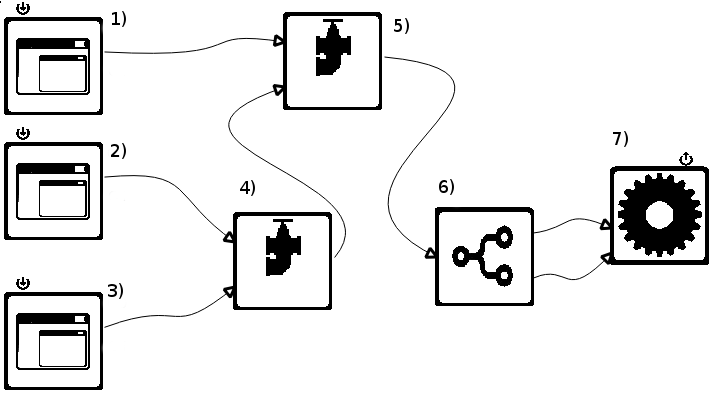
\includegraphics[width=3.5in]{3layers.png}
	\caption{Controller code with three competencies level. 1 --- Human control level. 2 --- Collision avoidance level. 3 --- Wandering level. 4 --- $Supressor$ block for levels 2,3. 5 --- $Supressor$ block for levels 1 and  2,3. 6 --- $Unzip$ block.  7 --- $Motors$ block.}
	\label{image:3layers}
\end{figure}

Each level is the simple robot controller without direct connection to actuators. Wandering (first level) continuously generates random number for each robot actuator, and sends its outside as array (see Figure ~\ref{image:1l}). The execution of this level starts with $InPort$ which emits data to activate two $RandomValue$ blocks. Each $RandomValue$ generate random number and emits it to $Wait$ block which after some predefined delay sends it to $Zip$ block which produces an array storing output values.

\begin{figure}[ht]
	\centering
	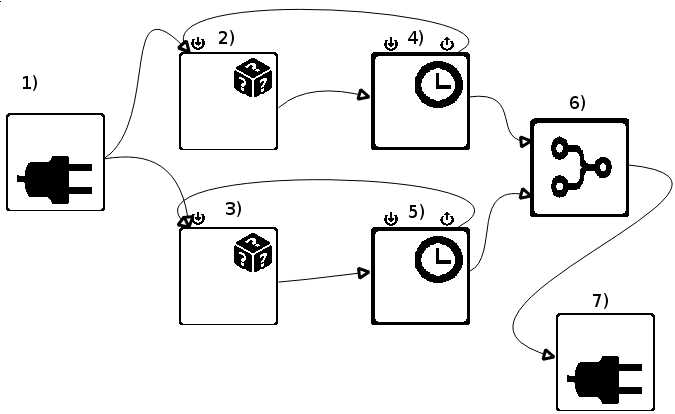
\includegraphics[width=3.5in]{1l.png}
	\caption{Walking. 1 --- $InPort$ block.  2,3 --- $RandomValue$ blocks. 4,5 --- $Wait$ blocks. 6 --- $Zip$ block. 7 --- $OutPort$ block.}
	\label{image:1l}
\end{figure}

The second level is needed to prevent collisions (see Figure ~\ref{image:2l}). It continuously gathers data by $Zip$ from two infrared $Sensors$ and checks if collision threatens (continuously after some delay by $DelayAndFilter$). If the collision can occur values sent for actuators to evade obstacles are calculated by $Function$. $Function$ block emits it to $Zip$ block which produces an array storing output values.

\begin{figure}[ht]
	\centering
	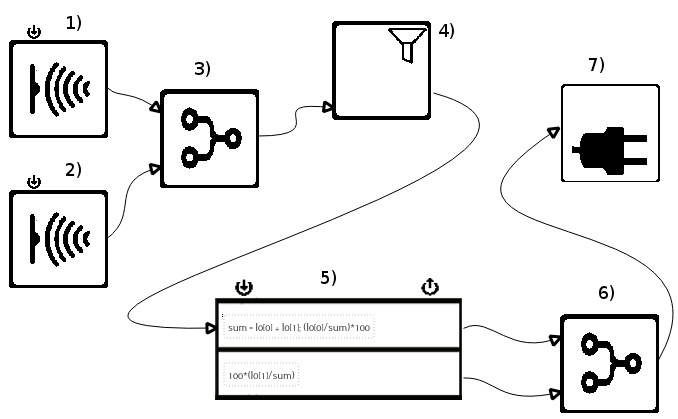
\includegraphics[width=3.5in]{2l.png}
	\caption{Collision avoidance. 1,2 --- $Sensor$ blocks. 3,6 --- $Zip$ block. 4 --- $DelayAndFilter$ block. 5 --- $Function$ block. 7 --- $OutPort$ block.}
	\label{image:2l}
\end{figure}

The third level is responsible for gamepad control. $Gamepad$ emits tokens describing current joystick and buttoins state. For simplicity we assume that pressing any button on gamepad will terminate the robot control program (by $FinalBlock$). The tokens are converted from the $Gamepad$ to the array of pulses for actuators by $Function$ block, which emits it through $OutPort$ block.

\begin{figure}[ht]
	\centering
	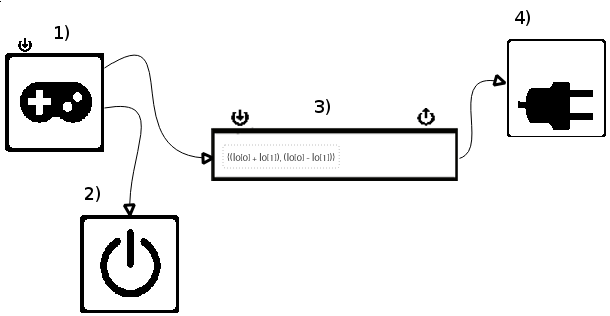
\includegraphics[width=3.5in]{3l.png}
	\caption{Human control. 1 --- $Gamepad$ block. 2 --- $FinalBlock$. 3 --- $Function$ block. 4 --- $OutPort$ block.}
	\label{image:3l}
\end{figure}


\section{Implementation}
\label{sec:Implementation}
The system is implemented as two plugins for TRIK Studio. The first one describes the visual language and provides visual editor for our system. It contains the metamodel of dataflow visual language and entirely generated by QReal DSM-platform. Plugged into TRIK Studio this module provides fully operational visual editor with all advantages of TRIK Studio control flow editor like modern-looking user interface, ability to create elements with mouse gestures, different appearances of links and so on. The time spent on the development of this plugin (not considering discussing and designing the prototype of visual language on paper) roughly equals three man-days. The benefit on exploiting the DSM-aproach is obviuos, the development of the similar editor from scratch would have been taken vastly more time.

The second plugin contains implementation of dataflow diagrams interpreter. Given the program drawn in editor (provided by first plugin) interpreter will transform that program into a sequence of the commands sent to a target robot (see fig.~\ref{image:common-architecture}). The target robot can be one of the supported in TRIK Studio infrasctructure: Lego NXT or EV3 robot, TRIK robot, TRIK Studio 2D simulator or $V\mbox{-}REP$ 3D simulator\cite{rohmer2013v}. Commands are sent via high-level TRIK Studio devices API, a part of it presented at fig.~\ref{image:devices-architecture}.

\begin{figure}[ht]
	\centering
	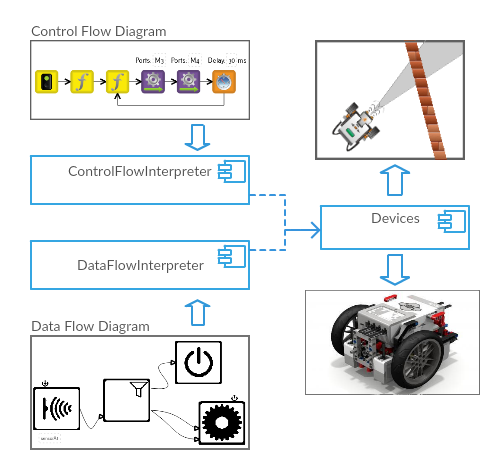
\includegraphics[width=3.5in]{Common.png}
	\caption{The general acrhitecture of the system}
	\label{image:common-architecture}
\end{figure}

\begin{figure}[ht]
	\centering
	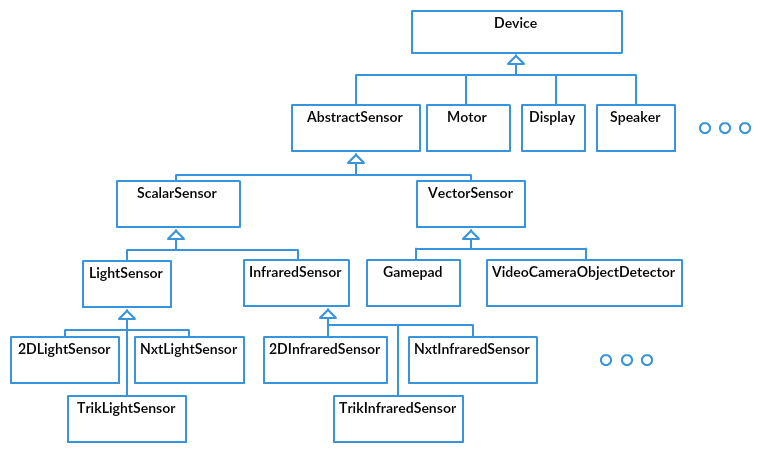
\includegraphics[width=3.5in]{Devices.png}
	\caption{Partial architecture of devices used in dataflow interpreter}
	\label{image:devices-architecture}
\end{figure}

The general acrhitecture of intepreter plugin is presented at fig.~\ref{image:interpreter-architecture}. Given dataflow diagram interpreter traverses, validates and prepares it for interpretation process. For each visited dataflow block implementation object is instantiated. Implementation objects are written in c++. Instantiation is performed by corresponding factory object. Implementation objects are then subscribed each to other like they are connected by flows on diagram, \textit{publish-subscribe} pattern is used here. The set of initial blocks is determined next, those are blocks without incomming flows. After all that done preparation phase is complete and diagram starts beeing interpreted.

\begin{figure}[ht]
	\centering
	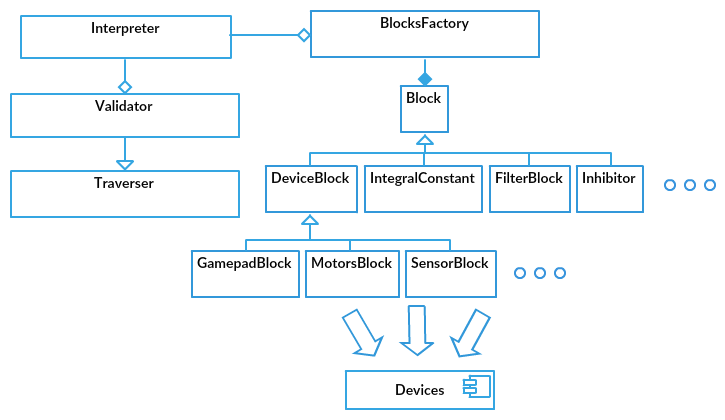
\includegraphics[width=3.5in]{Interpreter.png}
	\caption{The general architecture of dataflow interpreter plugin}
	\label{image:interpreter-architecture}
\end{figure}

Interpretation process is not as straightforward as in most asynchronious daflow environments. Usually components of dataflow diagram are executed concurrently, on different threads, processes or even machines (that is actively exploited, for example, by Microsoft Robotics Developer Studio where dataflow diagram is deployed into a number of web-services). That is a pretty convenient way to invoke dataflow diagrams on a powerful hardware, but not a case when we talk about embedded devices. In our case we deal exactly with embedded devices (Lego NXT, EV3, TRIK, Arduino controllers), so we propose here another way of executing dataflow diagrams. The main idea is to introduce global message queue and event loop for messages processing. When token is published by some block it is enqueued into messages queue and waits for its turn to be delivered to subscribers (fig.~\ref{image:interpreter-interaction}). In fact thus we \textit{flatten} the execution, convert concurrent way of dataflow interpretation to a pseudo-concurrent one where we schedule invocation order on our own. It must be noted that this mechanism is similar to events propagation system of Qt framework. That is actively exploited in our implementation, where message processing is completely performed by $QEventLoop$ class and tokens delivering is done by Qt signal/slot system in $QueuedConnection$ mode. 

Flat execution of dataflow diagram poses a number of small problems, one of them will be discussed here. Input device blocks (for example blocks publishing tokens from ultrasonic sensors) are constantly emitting tokens to subscribers. Subscribers transmit tokens to a next one (possibly in modified state) and so on. Thus there appears a chain of data processing. In our language that chain can activate control flow ports of blocks ``reviving'' them, so the control flow model is implicitly supported in out language (this is important in educational reasons). If later in this chain same input device block will be met then execution will come in a 
counterintuitive way. Such conflicts are ruled out with a simple heruistic that among all the blocks sharing one physical device only one can be active and that is the last activated one. Thus when the execution token comes into some device block it immediately ``deactivates'' conflicting ones. Other problems like messages balancing (in case when some block ``flooding'' the whole messages queue) will not be discussed here.

The last thing we should remark here is the presence of $Fork$ block in our language that usually is not provided by dataflow languages. Flattened model seems to work well on embedded devices, but sometimes users still need to use concurrent execution (for example for executing layers in Subsumption architecture). For that reason $Fork$ block is introduced, it forks the execution into a number of platform-specific execution units (for example $pthreads$ on UNIX or $tasks$ on NXT OSEK). This block can be regarded as low-level control of execution process. It should be also marked that this block almost has no sence in interpretation mode (because execution itself is performed on desktop machine with only sending primitive commands to robot), but will be very useful in future works when autonomous mode will be introduced.

\begin{figure}[ht]
	\centering
	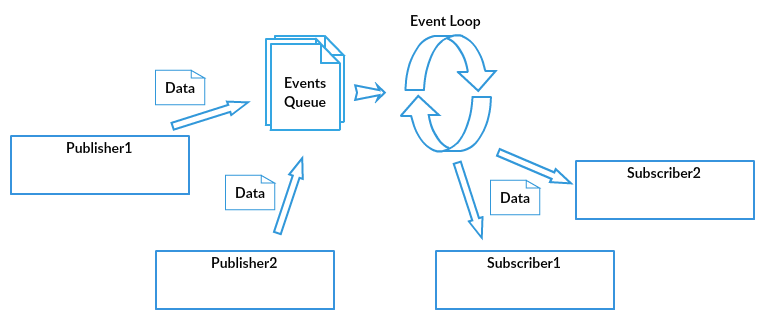
\includegraphics[width=3.5in]{Interaction.png}
	\caption{Proposed mechanism of pseudo-concurrent dataflow interpretation}
	\label{image:interpreter-interaction}
\end{figure}


\section{Conclusion and Discussion}
\label{sec:Conclusion}
In this work we presented the prototype of dataflow language for programming different robotic kits (LEGO MINDSTORMS NXT, LEGO MINDSTORMS EV3, TRIK). The system provides ability to interpret diagrams on 2D- an 3D-simulators and real robotic devices. Proposed an aproach for executing dataflow diagrams on embedded devices. The language implicitly supports control flow model for educational purposes. It is also convenient for expressing typical robotic controllers architectures which is demostrated on example.

The implemented system can be regarded as a platform for future investigations. First of all autonomious mode of work will be implemented. That will be done through code generation into a number of textual languages aready supported by TRIK Studio (NXT OSEK C for Lego, bytecode for EV3, JavaScript, F\#\cite{kirsanov2014robotics} and Kotlin for TRIK). We are also interested in academical research. First of all a formal semantics of our language should be expressed for applying various formal methods of program analysis. Another branch of research will be directed into a DSM-branch, here we want to consider an ability of dynamic langiage metamodel generation from specifications of available modules of robotics middleware (like ROS\cite{quigley2009ros} or Player\cite{gerkey2003player}).

\newpage
\bibliography{IEEEbibl}
\bibliographystyle{IEEEtran}
\end{document}
